\section{Materiales y métodos}

\subsection{Materiales}

\subsection{Metodología}

EL flujo de trabajo que se siguió puede observarse en la figura \ref{fig:workflow} y que se explicará en detalle a continuación.

\begin{figure}[h!]
	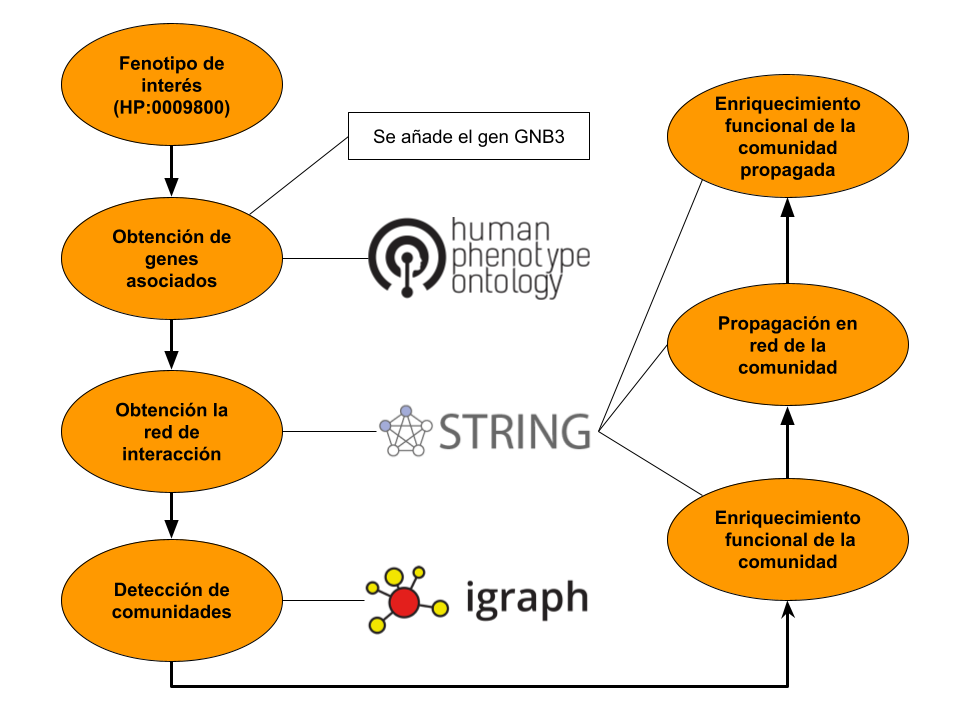
\includegraphics[width=0.9\textwidth]{figures/workflow.png}
	\caption{Flujo de trabajo: Se representa el flujo de trabajo seguido para la realización del proyecto. Empieza desde la obtención de los genes asociados al fenotipo de interés y la creación de la red de interacción hasta el análisis por enriquecimiento funcional.}
	\label{fig:workflow}
\end{figure}

Descargamos la lista de genes implicados al fenotipo HP:0009800 directamente desde HPO en formato excel.

Utilizamos la librería de Python de stringdb mediante el método "get\_network" para realizar una petición a su API para obtener la red de interacción de los genes asociados al fenotipo a la que previamente se insertó el gen GNB3 para realizar su estudio.

Mediante la librería de igraph se construyó la red de interacción de genes y se realizó un algoritmo de detección de comunidades basado en "edge betweenness". Una vez realizado la detección, se seleccionó la comunidad donde estaba presente el gen GNB3.

Realzamos un enriquecimiento funcional de los genes que formaban parte de esa comunidad mediante la librería de stringdb mediante el método "get\_enrichment". 

Se creó una nueva red mediante una propagación en red de los genes presente en la comunidad de interés a través del método "get\_network" con un nuevo parámetro de entrada "add\_nodes = 16" para indicar que se añadieron 16 genes más. A partir de esta red volvimos a realizar un enriquecimiento funcional.
